\documentclass{article}
\usepackage[T1]{fontenc}
\usepackage[latin2]{inputenc}
\usepackage[english]{babel}
\usepackage{tikz}
\usepackage{times}
\usetikzlibrary{calc,through,backgrounds,positioning,fit}
\usetikzlibrary{shapes,arrows,shadows,calendar}
 
\begin{document}

 
\centering
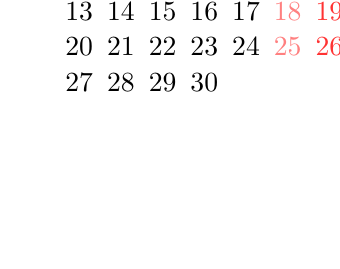
\begin{tikzpicture}[scale=1,inner sep=0.4mm]
\tikz
\calendar
[dates=2015-04-01 to 2015-04-30,week list,month label above centered, month text=\%mt \%y0]
if (equals = 2015-04-06)[red]
if (Saturday) [red!50]
if (Sunday) [red!80];

\end{tikzpicture}
 
\end{document}